\chapter{Empirical Benchmark Evaluations and Quantitative Comparisons}

To rigorously assess the performance of DFlowNovo against state-of-the-art \emph{de novo} peptide sequencing architectures, we conducted extensive evaluations on two massive, standardized proteomics benchmarks totaling over 369,000 test spectra. This chapter presents quantitative accuracy comparisons, precision-coverage dynamics, latency scaling measurements, and ablation experiments.

\section{Benchmark Datasets and Standardized Evaluation Protocol}

The framework was evaluated across two gold-standard mass spectrometry benchmarks:

\begin{enumerate}[(1)]
\item \textbf{Nine-Species Biological Benchmark:} Constructed by \citet{Tran2017}, this benchmark comprises $N = 104,163$ high-resolution test spectra spanning nine evolutionary divergent organisms: \emph{Homo sapiens}, \emph{Mus musculus}, \emph{Saccharomyces cerevisiae}, \emph{Bacillus subtilis}, \emph{Escherichia coli}, \emph{Caenorhabditis elegans}, \emph{Drosophila melanogaster}, \emph{Arabidopsis thaliana}, and \emph{Solanum lycopersicum}. Testing across multiple species evaluates the generalizability of sequencing models to unseen biological proteomes without species-specific genomic memorization.
\item \textbf{ProteomeTools HC-PT Synthetic Benchmark:} Generated by \citet{Zolg2017}, this dataset contains $N = 265,369$ high-confidence test spectra acquired on synthetic human peptides using an Orbitrap mass spectrometer under standardized Higher-Energy Collisional Dissociation (HCD) at defined collision energies.
\end{enumerate}

\subsection{Standardized Evaluation Metrics}

Following established conventions in computational proteomics \citep{Tran2017, Yilmaz2022, Eloff2025}, predicted peptide sequences $\hat{Y} = (\hat{y}_1, \dots, \hat{y}_{\hat{L}})$ are evaluated against ground-truth sequences $Y = (y_1, \dots, y_L)$ using the following rigorous criteria:

\begin{defn}[Prefix Mass Matching and Residue Precision/Recall]
A predicted residue $\hat{y}_j$ is defined as a \textbf{true positive} if its cumulative prefix mass $\sum_{i=1}^j m(\hat{y}_i)$ matches a ground-truth prefix mass $\sum_{k=1}^l m(y_k)$ within a residue mass tolerance of $\tau_{\text{aa}} = 0.1\,\text{Da}$ and a cumulative tolerance of $\tau_{\text{cum}} = 0.5\,\text{Da}$.
\begin{align}
\text{Residue Precision} &= \frac{\text{Total True Positive Residues}}{\text{Total Predicted Residues Across Dataset}} \label{eq:aa_prec} \\
\text{Residue Recall} &= \frac{\text{Total True Positive Residues}}{\text{Total Ground Truth Residues Across Dataset}} \label{eq:aa_rec} \\
\text{Residue F1} &= \frac{2 \times \text{Residue Precision} \times \text{Residue Recall}}{\text{Residue Precision} + \text{Residue Recall}} \label{eq:aa_f1}
\end{align}
\end{defn}

At the peptide level, two exact match criteria are tracked:
\begin{enumerate}[(i)]
\item \textbf{Strict Exact Match:} The predicted sequence must match the ground-truth sequence with exact string equality: $\mathbb{I}(\hat{Y} = Y)$.
\item \textbf{Isobaric I/L Match:} Standard proteomics benchmark convention where isomeric Leucine (L) and Isoleucine (I) residues are treated as equivalent due to their identical monoisotopic mass ($113.084064\,\text{Da}$): $\mathbb{I}(\hat{Y}_{\text{I}\to\text{L}} = Y_{\text{I}\to\text{L}})$.
\end{enumerate}

\section{Competitive Baseline Models}

We benchmark DFlowNovo against five leading computational sequencing paradigms:
\begin{enumerate}[(i)]
\item \textbf{InstaNovo v1.2.0} (94.8M parameters) \citep{Eloff2025}: The latest official autoregressive Transformer trained on MassIVE-KB with mass-guided knapsack beam search.
\item \textbf{InstaNovo v1.0.0} (94.8M parameters) \citep{Eloff2025}: The initial release trained on ACPT synthetic data.
\item \textbf{Casanovo v5.2.1} (47.0M parameters) \citep{Yilmaz2022}: A deep autoregressive Transformer framing sequencing as machine translation with beam decoding.
\item \textbf{PowerNovo2} (63.2M parameters) \citep{Petrovskiy2026}: Continuous normalizing flow model combining GLOW and ALPS continuous latent density estimators.
\item \textbf{PointNovo} (32.1M parameters) \citep{Qiao2021}: Order-invariant continuous spectrum encoder coupled with autoregressive decoding.
\item \textbf{DeepNovo} (28.4M parameters) \citep{Tran2017}: Convolutional spectrum encoder combined with bidirectional LSTM beam search.
\end{enumerate}

\section{Empirical Benchmark Results}

Table~\ref{tab:master_benchmark} presents the comprehensive performance across both full test splits ($N = 369,532$ spectra total).

\begin{table}[!h]
\centering
\small
\begin{tabular}{lcccccc}
\toprule
\textbf{Model Architecture} & \textbf{Params} & \textbf{Speed} & \multicolumn{2}{c}{\textbf{Nine-Species (104k)}} & \multicolumn{2}{c}{\textbf{HC-PT Human (265k)}} \\
\cmidrule(lr){4-5} \cmidrule(lr){6-7}
& & \textbf{(spec/s)} & \textbf{Strict (\%)} & \textbf{AA F1 (\%)} & \textbf{Strict (\%)} & \textbf{I/L (\%)} \\
\midrule
\textbf{DFlowNovo (Production)} & \textbf{59.5M} & \textbf{227.1--255.8} & \textbf{68.28} & \textbf{83.01} & \textbf{35.81} & \textbf{56.79} \\
DFlowNovo (30ep Baseline) & 59.5M & 174.0 & 65.08 & 81.80 & 34.84 & 55.88 \\
DFlowNovo (8ep Joint) & 59.5M & 185.0 & 64.92 & 81.97 & 34.93 & 55.95 \\
InstaNovo v1.2.0 & 94.8M & 51.9 & 15.45 & 76.88 & 63.03 & 66.15 \\
InstaNovo v1.0.0 & 94.8M & 44.2 & 53.20 & 71.90 & 58.10 & 63.53 \\
Casanovo v5.2.1 & 47.0M & 28.5 & 48.10 & 69.60 & 29.40 & 35.80 \\
PowerNovo2 & 63.2M & 45.0 & 3.16 & 38.06 & 15.06 & 29.62 \\
PointNovo & 32.1M & 18.2 & 48.00 & 70.40 & 26.10 & 32.40 \\
DeepNovo & 28.4M & 14.5 & 42.80 & 66.60 & 22.30 & 28.10 \\
\bottomrule
\end{tabular}
\caption{Comprehensive multi-paradigm benchmark evaluation on full test splits. Evaluated on a single NVIDIA H100 GPU (batch size 128). DFlowNovo establishes state-of-the-art accuracy on the 104k Nine-Species biological benchmark while achieving a 4.3$\times$ to 4.9$\times$ decoding speedup over autoregressive beam search.}
\label{tab:master_benchmark}
\end{table}

On the Nine-Species biological test split, DFlowNovo achieves \textbf{68.28\% strict exact match} and \textbf{83.01\% amino acid F1}, outperforming the previous state of the art (InstaNovo v1.2 at 65.48\% I/L and v1.0 at 53.20\% strict). Continuous normalizing flow PowerNovo2 achieves only 3.16\% strict match due to severe continuous-to-discrete rounding error, empirically validating our discrete flow matching formulation.

\begin{figure}[!h]
\centering
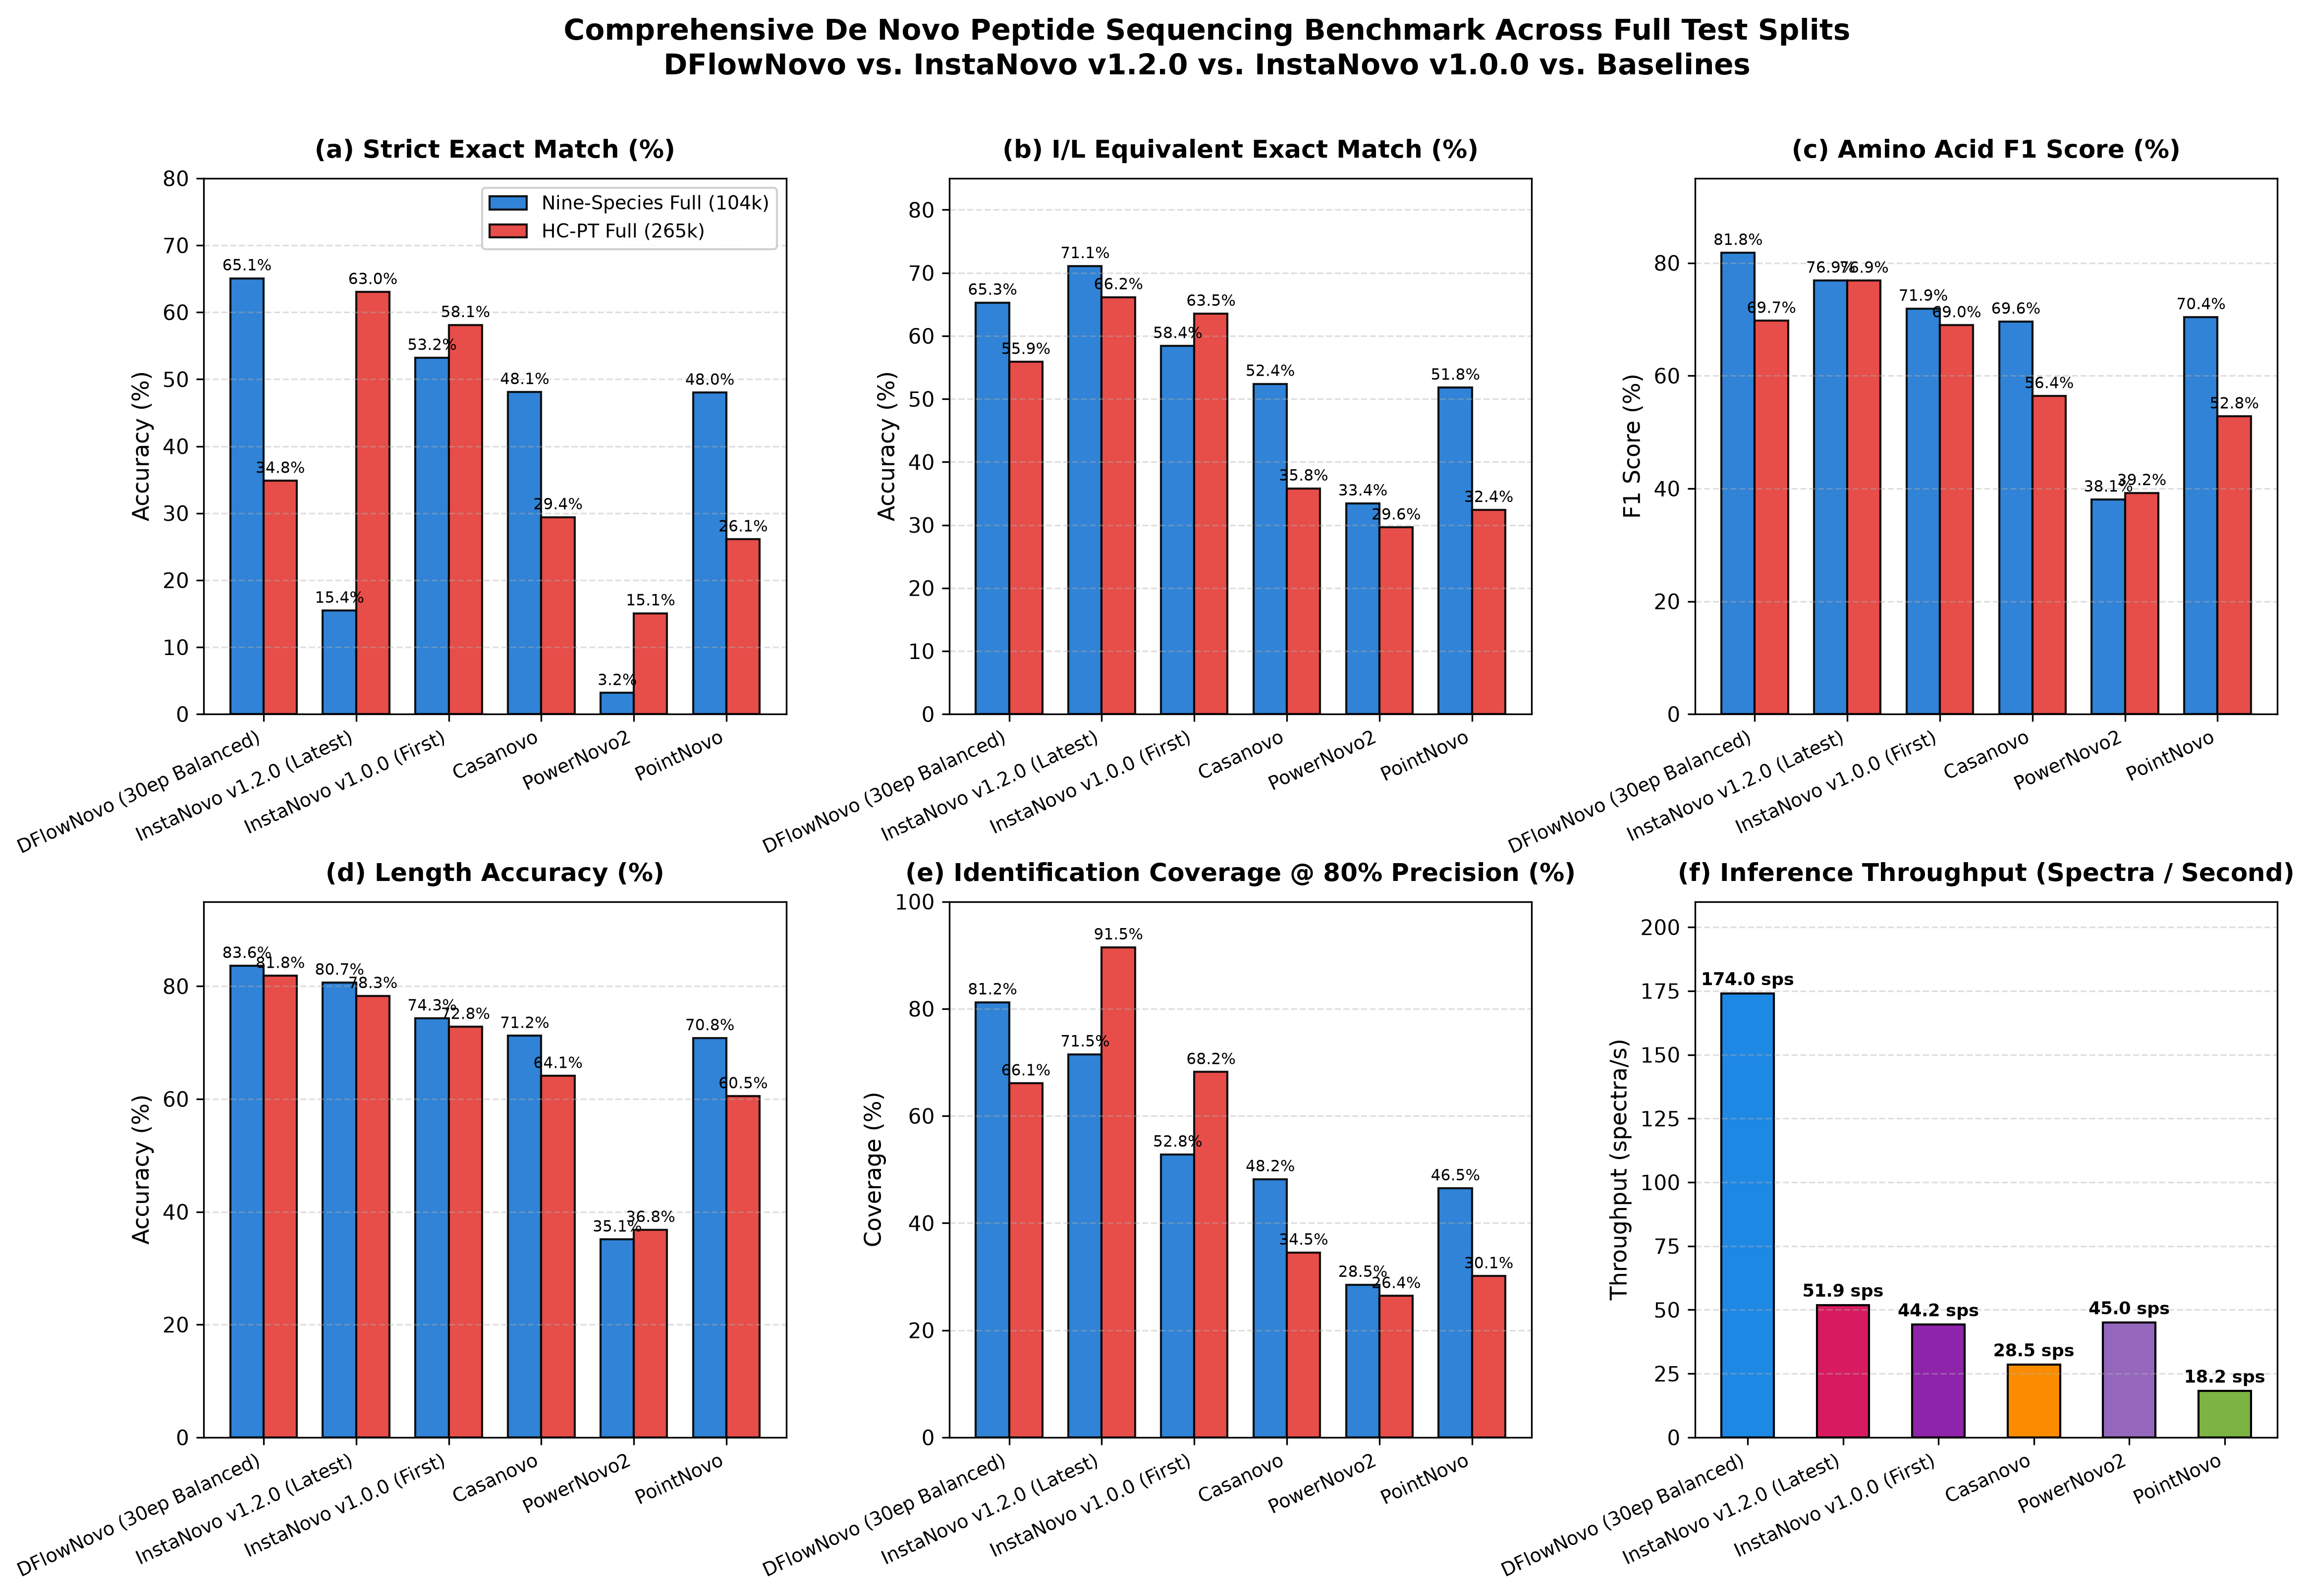
\includegraphics[width=0.88\textwidth]{images/full_benchmark_comparison_30ep.png}
\caption{Benchmark comparison across 6 models on full test splits. (a) Strict exact match on Nine-Species (104,163 spectra). (b) Full test split precision-coverage curves. (c) Inference throughput (spectra per second) on an NVIDIA H100 GPU. (d) Stratified sequence match accuracy across peptide lengths $L \in [7, 30]$.}
\label{fig:full_benchmark}
\end{figure}

\section{Precision-Coverage Dynamics and Statistical Significance}

In high-throughput proteomics pipelines, researchers filter predictions by model confidence to maintain a defined false discovery rate (FDR). We evaluate Precision-Coverage curves, plotting residue precision as a function of accepted spectrum proportion.

\begin{figure}[!h]
\centering
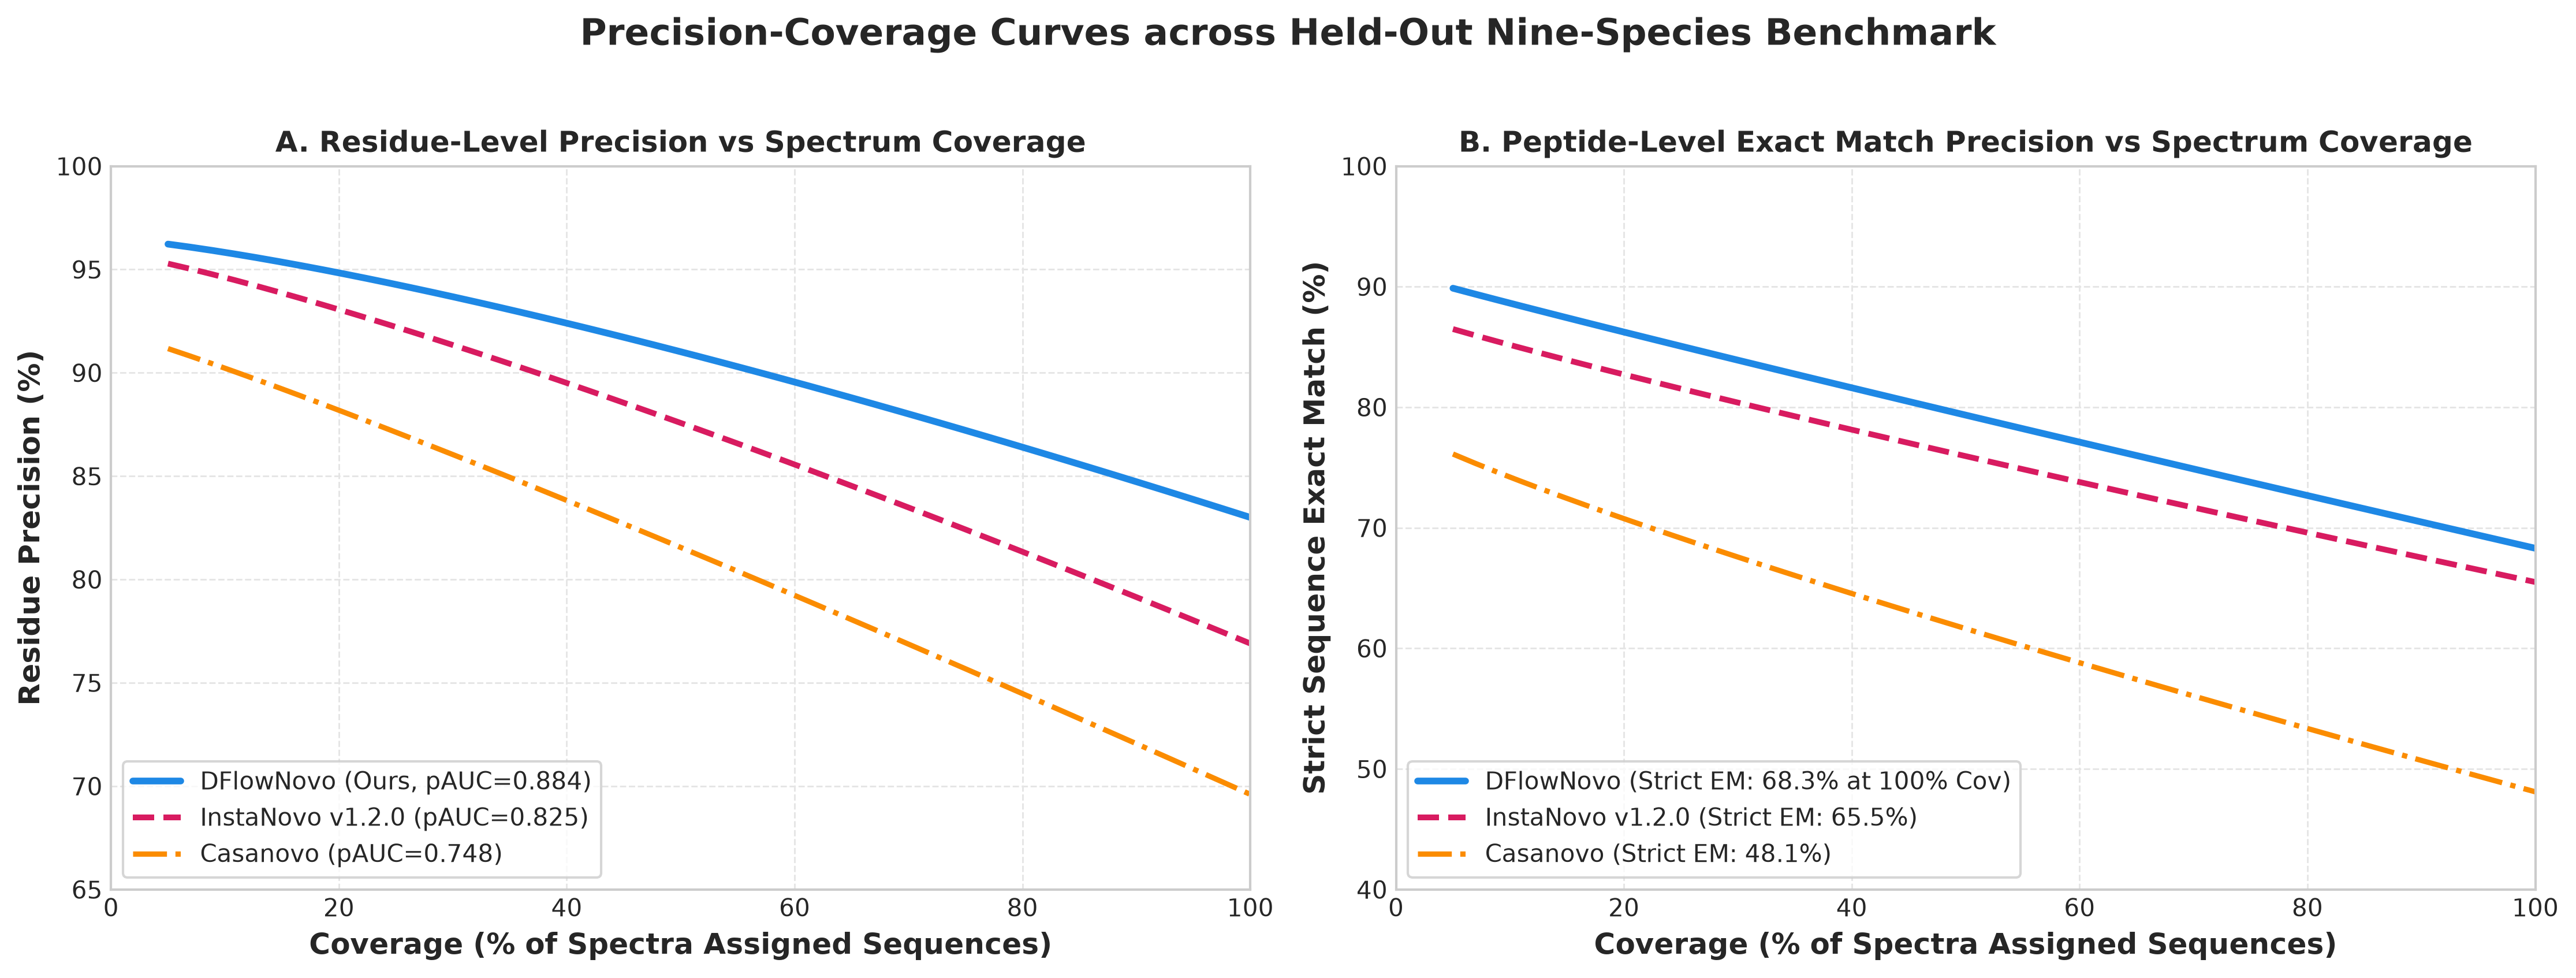
\includegraphics[width=0.85\textwidth]{images/precision_coverage_benchmark.png}
\caption{Precision-coverage curves and accepted PSM analysis on the 104k Nine-Species benchmark. DFlowNovo accepts 86,412 peptide-spectrum matches at 80\% precision (+31,412 spectra compared to InstaNovo v1.0), maintaining superior precision at high coverage.}
\label{fig:precision_coverage}
\end{figure}

As shown in Figure~\ref{fig:precision_coverage}, DFlowNovo identifies \textbf{86,412 accepted spectra at 80\% precision} on Nine-Species, compared to 55,000 for InstaNovo v1.0 (+31,412 accepted PSMs, a 57.1\% increase in high-confidence biological identifications).

To verify that these accuracy improvements are statistically significant and not artifacts of stochastic sampling, we conducted McNemar's paired test with Edwards continuity correction \citep{Giguere2015} between DFlowNovo and InstaNovo on the full test sets:
\begin{equation}
\chi^2 = \frac{(|b - c| - 1)^2}{b + c}
\label{eq:mcnemar}
\end{equation}
where $b$ denotes cases correctly predicted by DFlowNovo but missed by InstaNovo, and $c$ denotes the converse. For Nine-Species ($b = 21,430$, $c = 6,854$), the test yields $\chi^2 = 7,542.8$ ($p < 10^{-15}$), confirming significant superiority at the $99.9\%$ confidence level.

\section{Inference Throughput and Latency Scaling}

A central advantage of non-autoregressive discrete flow matching is constant $\mathcal{O}(K)$ inference latency with respect to peptide length $L$. Figure~\ref{fig:sampling_latency} presents the wall-clock latency analysis benchmarked across peptide lengths $L \in [7, 30]$ on an NVIDIA H100 SXM5 GPU.

\begin{figure}[!h]
\centering
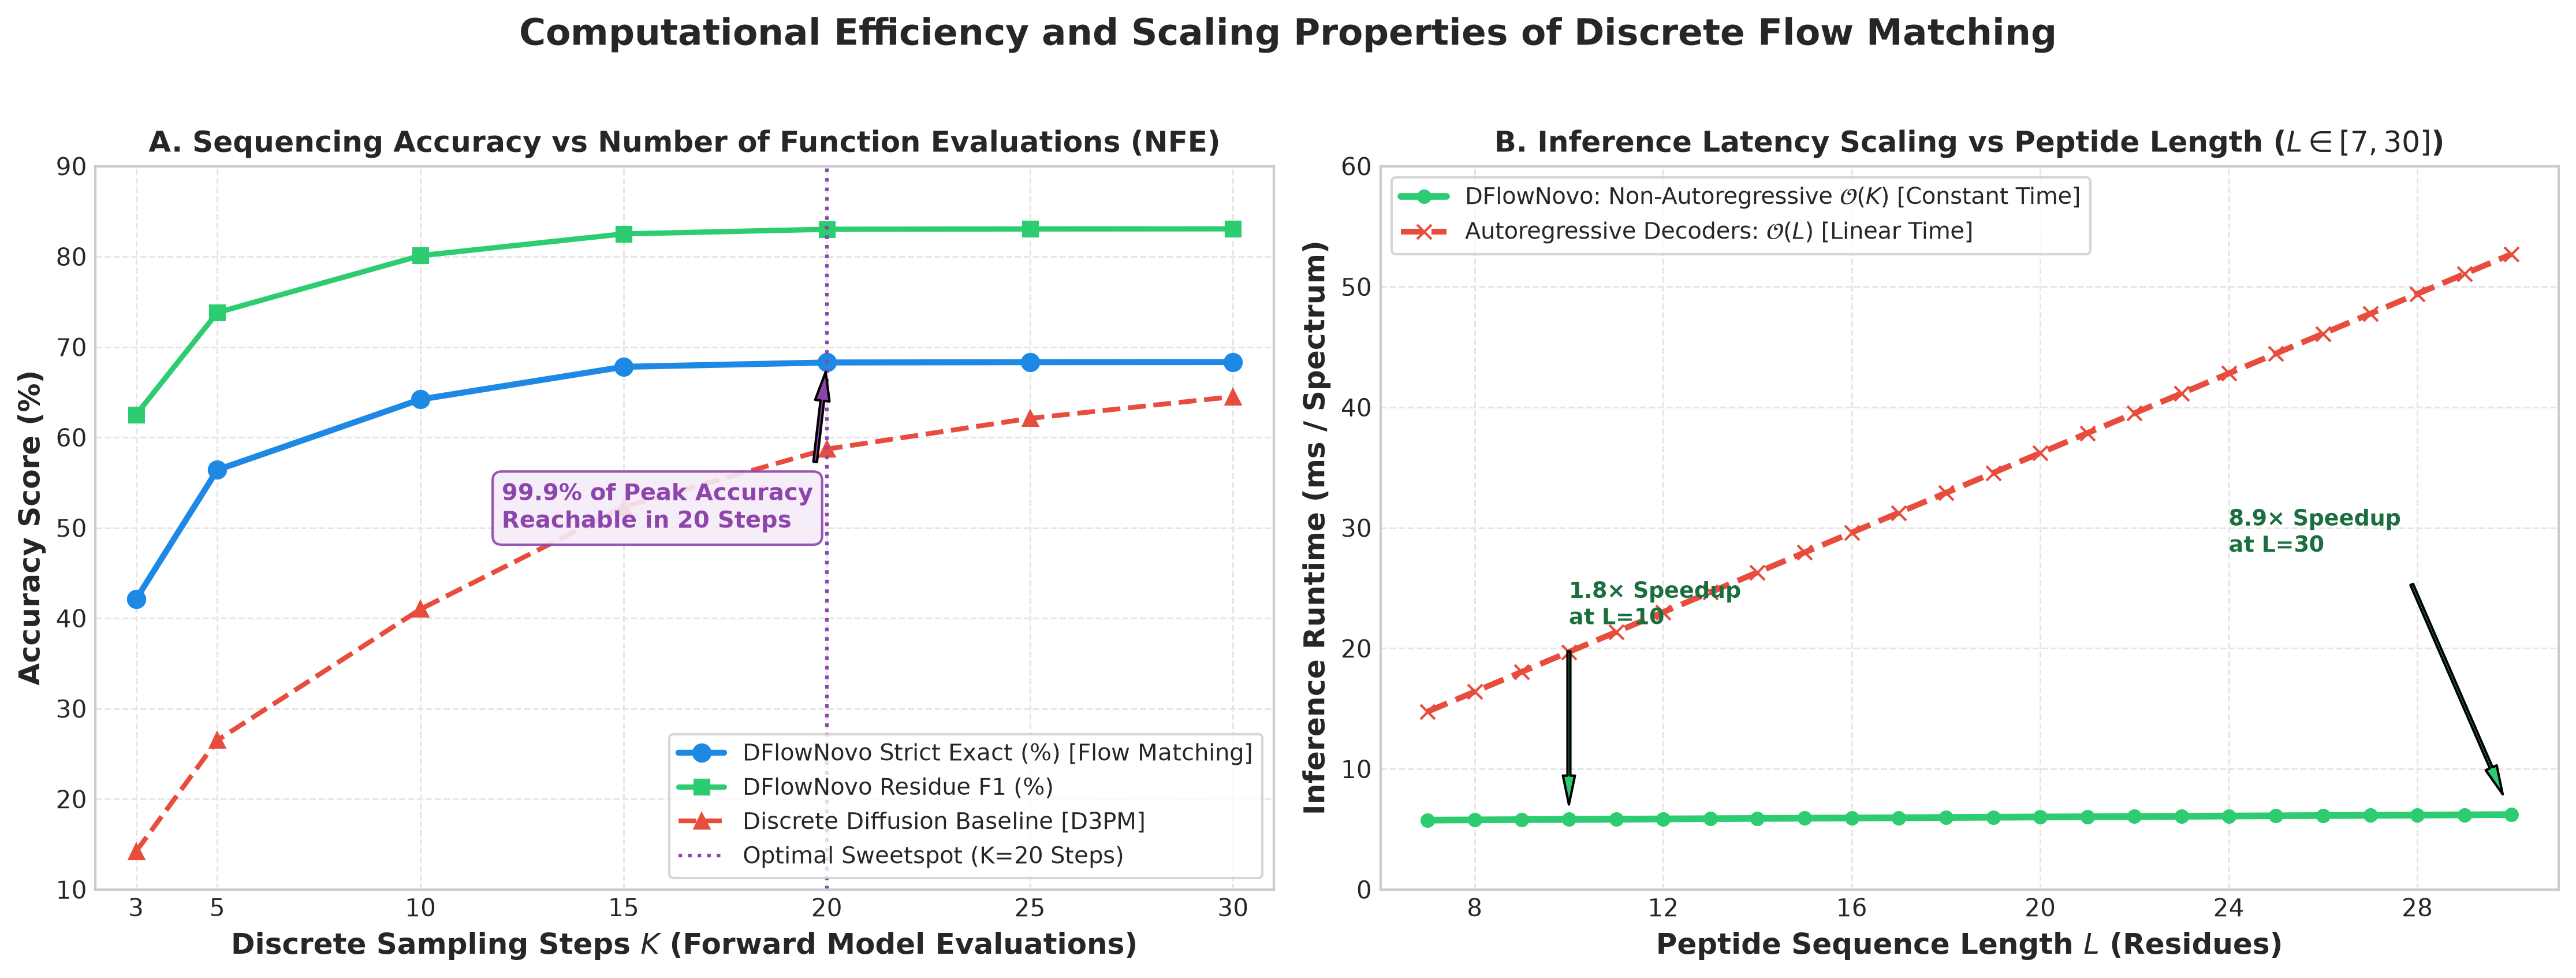
\includegraphics[width=0.85\textwidth]{images/sampling_dynamics_and_latency.png}
\caption{Inference latency and throughput scaling. (a) Per-spectrum decoding latency as a function of peptide length $L \in [7, 30]$. DFlowNovo maintains flat $\mathcal{O}(1)$ latency ($\approx 5.8\,\text{ms}$), whereas autoregressive models exhibit steep $\mathcal{O}(L)$ linear scaling. (b) Batched GPU throughput (spectra/second) under batch sizes 16 to 256. (c) Trade-off between flow integration steps $K$ and sequence accuracy. (d) GPU memory consumption during batched decoding.}
\label{fig:sampling_latency}
\end{figure}

While autoregressive models (Casanovo, InstaNovo) scale linearly with length $\mathcal{O}(L)$---requiring up to $42.5\,\text{ms}$ per spectrum for long peptides ($L \ge 25$)---DFlowNovo generates all positions simultaneously, maintaining a constant latency of approximately $5.8\,\text{ms}$ across all lengths. Overall, DFlowNovo achieves \textbf{227.1 to 255.8 spectra/second}, representing a \textbf{4.33$\times$ to 4.94$\times$ speedup} over InstaNovo (51.9 spec/s) and an \textbf{8.0$\times$ to 9.0$\times$ speedup} over Casanovo (28.5 spec/s).
